% !TEX program = xelatex

\documentclass{beamer}
\usepackage[utf8]{inputenc}
\usepackage{xeCJK}
\usepackage{utopia} %font utopia imported
%\usepackage[UTF8,noindent]{ctexcap}
\usetheme{Rochester}
\usecolortheme{default}
 % 衬线字体:Linux Libertine
    % BoldFont 可以选择 Bold 字重或者 Semibold 字重
    % BoldItalicFont 也有对应 BoldFont 的字重选择
    % 这里使用 Semibold 字重
  %   \setmainfont{LinLibertine_R.otf}[
  %     BoldFont = LinLibertine_RZ.otf,
  %     ItalicFont = LinLibertine_RI.otf,
  %     BoldItalicFont = LinLibertine_RZI.otf]
  % % % 无衬线字体:Linux Biolinum
  % \setsansfont{LinBiolinum_R.otf}[
  %     BoldFont = LinBiolinum_RB.otf,
  %     ItalicFont = LinBiolinum_RI.otf,
  %     BoldItalicFont = LinBiolinum_RBO.otf]
  % % 等宽/打印机字体:Linux Libertine Mono
  % \setmonofont{LinLibertine_M.otf}[
  %     BoldFont = LinLibertine_MB.otf,
  %     ItalicFont = LinLibertine_MO.otf,
  %     BoldItalicFont  = LinLibertine_MBO.otf]
  % \setCJKmainfont[ItalicFont={AR PL UKai CN},
  % BoldFont={WenQuanYi Micro Hei}]{IPAMinCho,IPA明朝}
  \setCJKsansfont{WenQuanYi Micro Hei}
  \setCJKmonofont{WenQuanYi Micro Hei Mono}
%------------------------------------------------------------
%This block of code defines the information to appear in the
%Title page
\title[光电中期报告] %optional
{光电子技术实验}

\subtitle{固体激光器的静态特性及调Q技术}

\author[芦, 王] % (optional)
{芦迪 \and 王莘景}

\institute[THU, EE] % (optional)
{

  Department of Electronic Engineering\\
  Tsinghua University
}

\date[2017.11.7] % (optional)
{\today}

\logo{
\includegraphics[height=1.5cm]{images/thuee-logo.png}}

%End of title page configuration block
%------------------------------------------------------------



%------------------------------------------------------------
%The next block of commands puts the table of contents at the 
%beginning of each section and highlights the current section:

\AtBeginSection[]
{
  \begin{frame}
    \frametitle{目录}
    \tableofcontents[currentsection]
  \end{frame}
}
%------------------------------------------------------------


\begin{document}

%The next statement creates the title page.
\frame{\titlepage}


%---------------------------------------------------------
%This block of code is for the table of contents after
%the title page
\begin{frame}
\frametitle{目录}
\tableofcontents
\end{frame}
%---------------------------------------------------------


\section{实验任务}

%---------------------------------------------------------
%Changing visivility of the text
\begin{frame}
\frametitle{实验任务}

本次实验的实验目的为:
\begin{enumerate}
  \item 掌握固体激光器与调 Q 工作原理
  \item 掌握固体激光器的调节方法,了解谐振腔参数及调节精度对激光器性能的影响
  \item 测量固体激光器的静态输出特性和调Q输出特性
  \item 掌握用于固体激光器调整和测量仪器的使用方法
\end{enumerate}
\end{frame}

\begin{frame}
  \frametitle{实验任务}
为达到以上目的,实验设计了如下任务: \\

\begin{enumerate}
    \item 装调固体激光器使之产生激光,反复调整降低阈值
    \item 测量固体激光器输出-输入能量关系曲线
    \item 观察激光器的静态输出波形,记录其波形与总宽度
    \item 测量固体激光器调Q输出波形,改变输入能量观察输出脉冲个数
    \item 测量固体激光器调Q输出-输入能量关系曲线并分析其特点
    \item 观测谐振腔调制精度对激光器的影响
\end{enumerate}
\end{frame}

%---------------------------------------------------------


%---------------------------------------------------------
%Example of the \pause command
% \begin{frame}
%   \frametitle{实验原理}
% In this slide \pause

% the text will be partially visible \pause

% And finally everything will be there
% \end{frame}
%---------------------------------------------------------

\section{实验原理}

%---------------------------------------------------------
%Highlighting text
\begin{frame}{实验原理}{固体激光器工作原理}
% \frametitle
固体激光器的结构如图:
\begin{figure}
  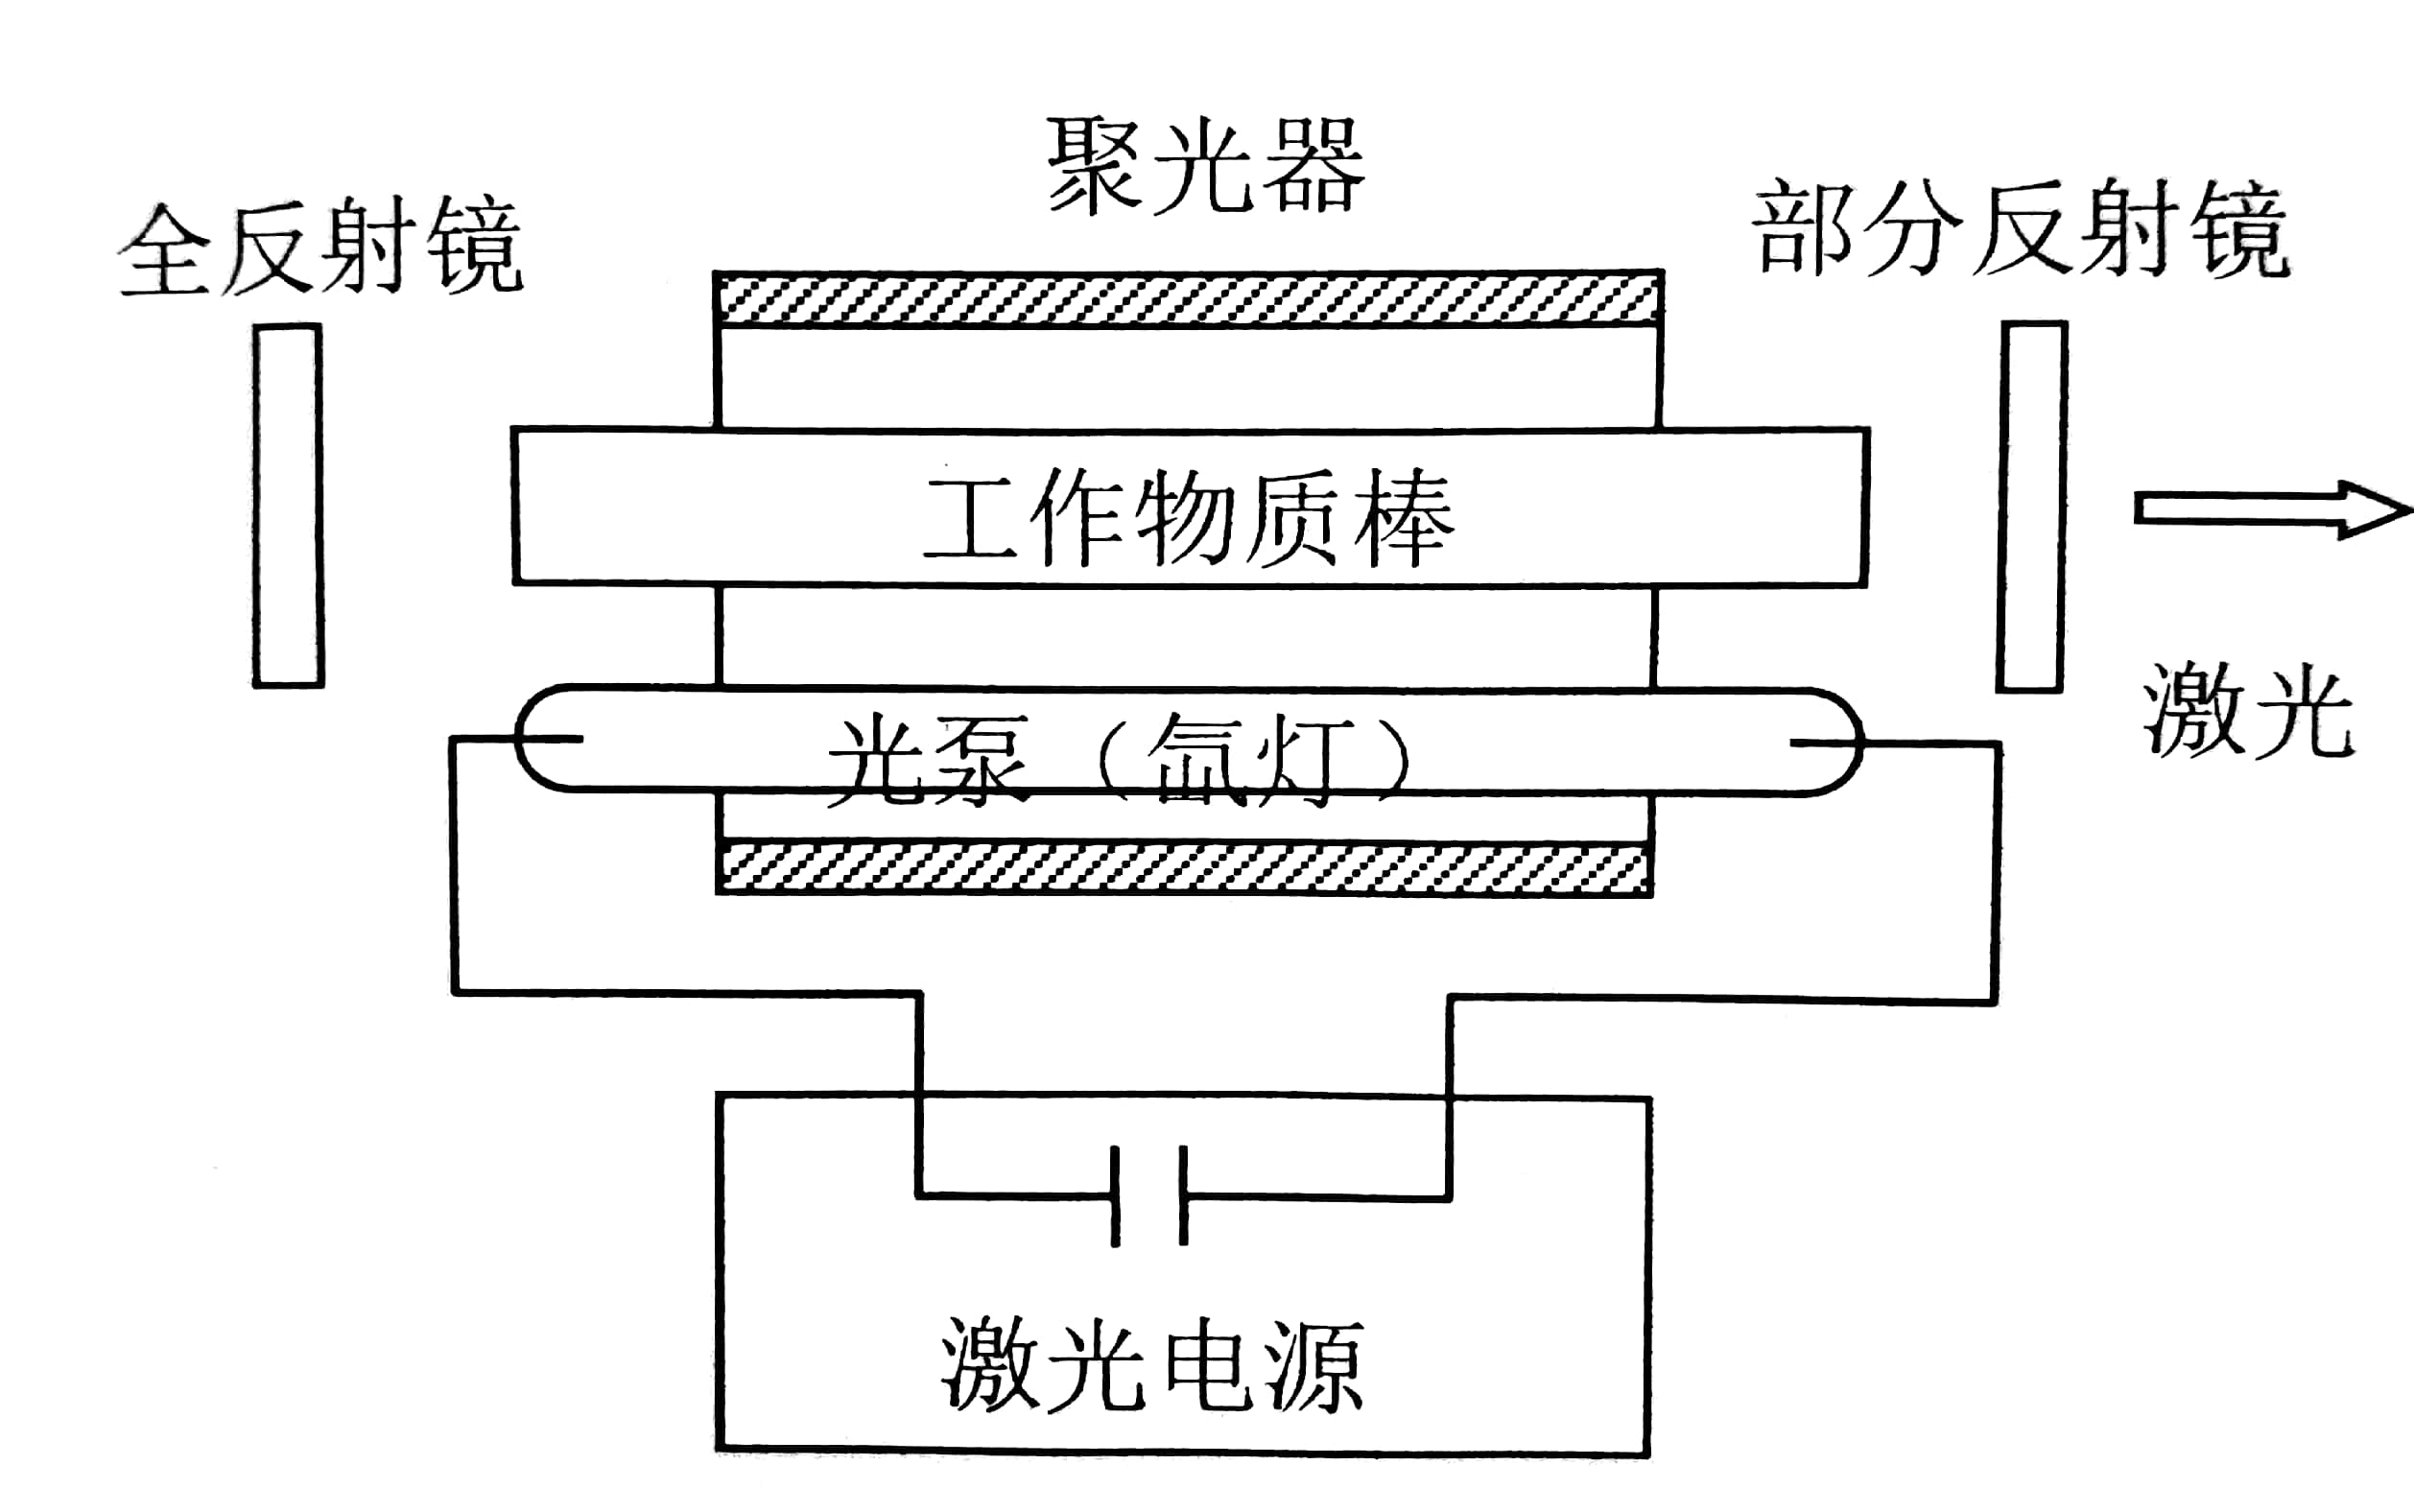
\includegraphics[height=3cm,width=5cm]{images/1.jpg}
  \label{fg1}
\end{figure}
本实验采用的工作物质为 \(\rm Nd:YAG\),激活离子为\(\rm Nd^{3+}\),激光输出波长为\(1.06\mu m\)。
\end{frame}
\begin{frame}{实验原理}{固体激光器工作原理}
  钕离子的能级示意图为:
  \begin{figure}
    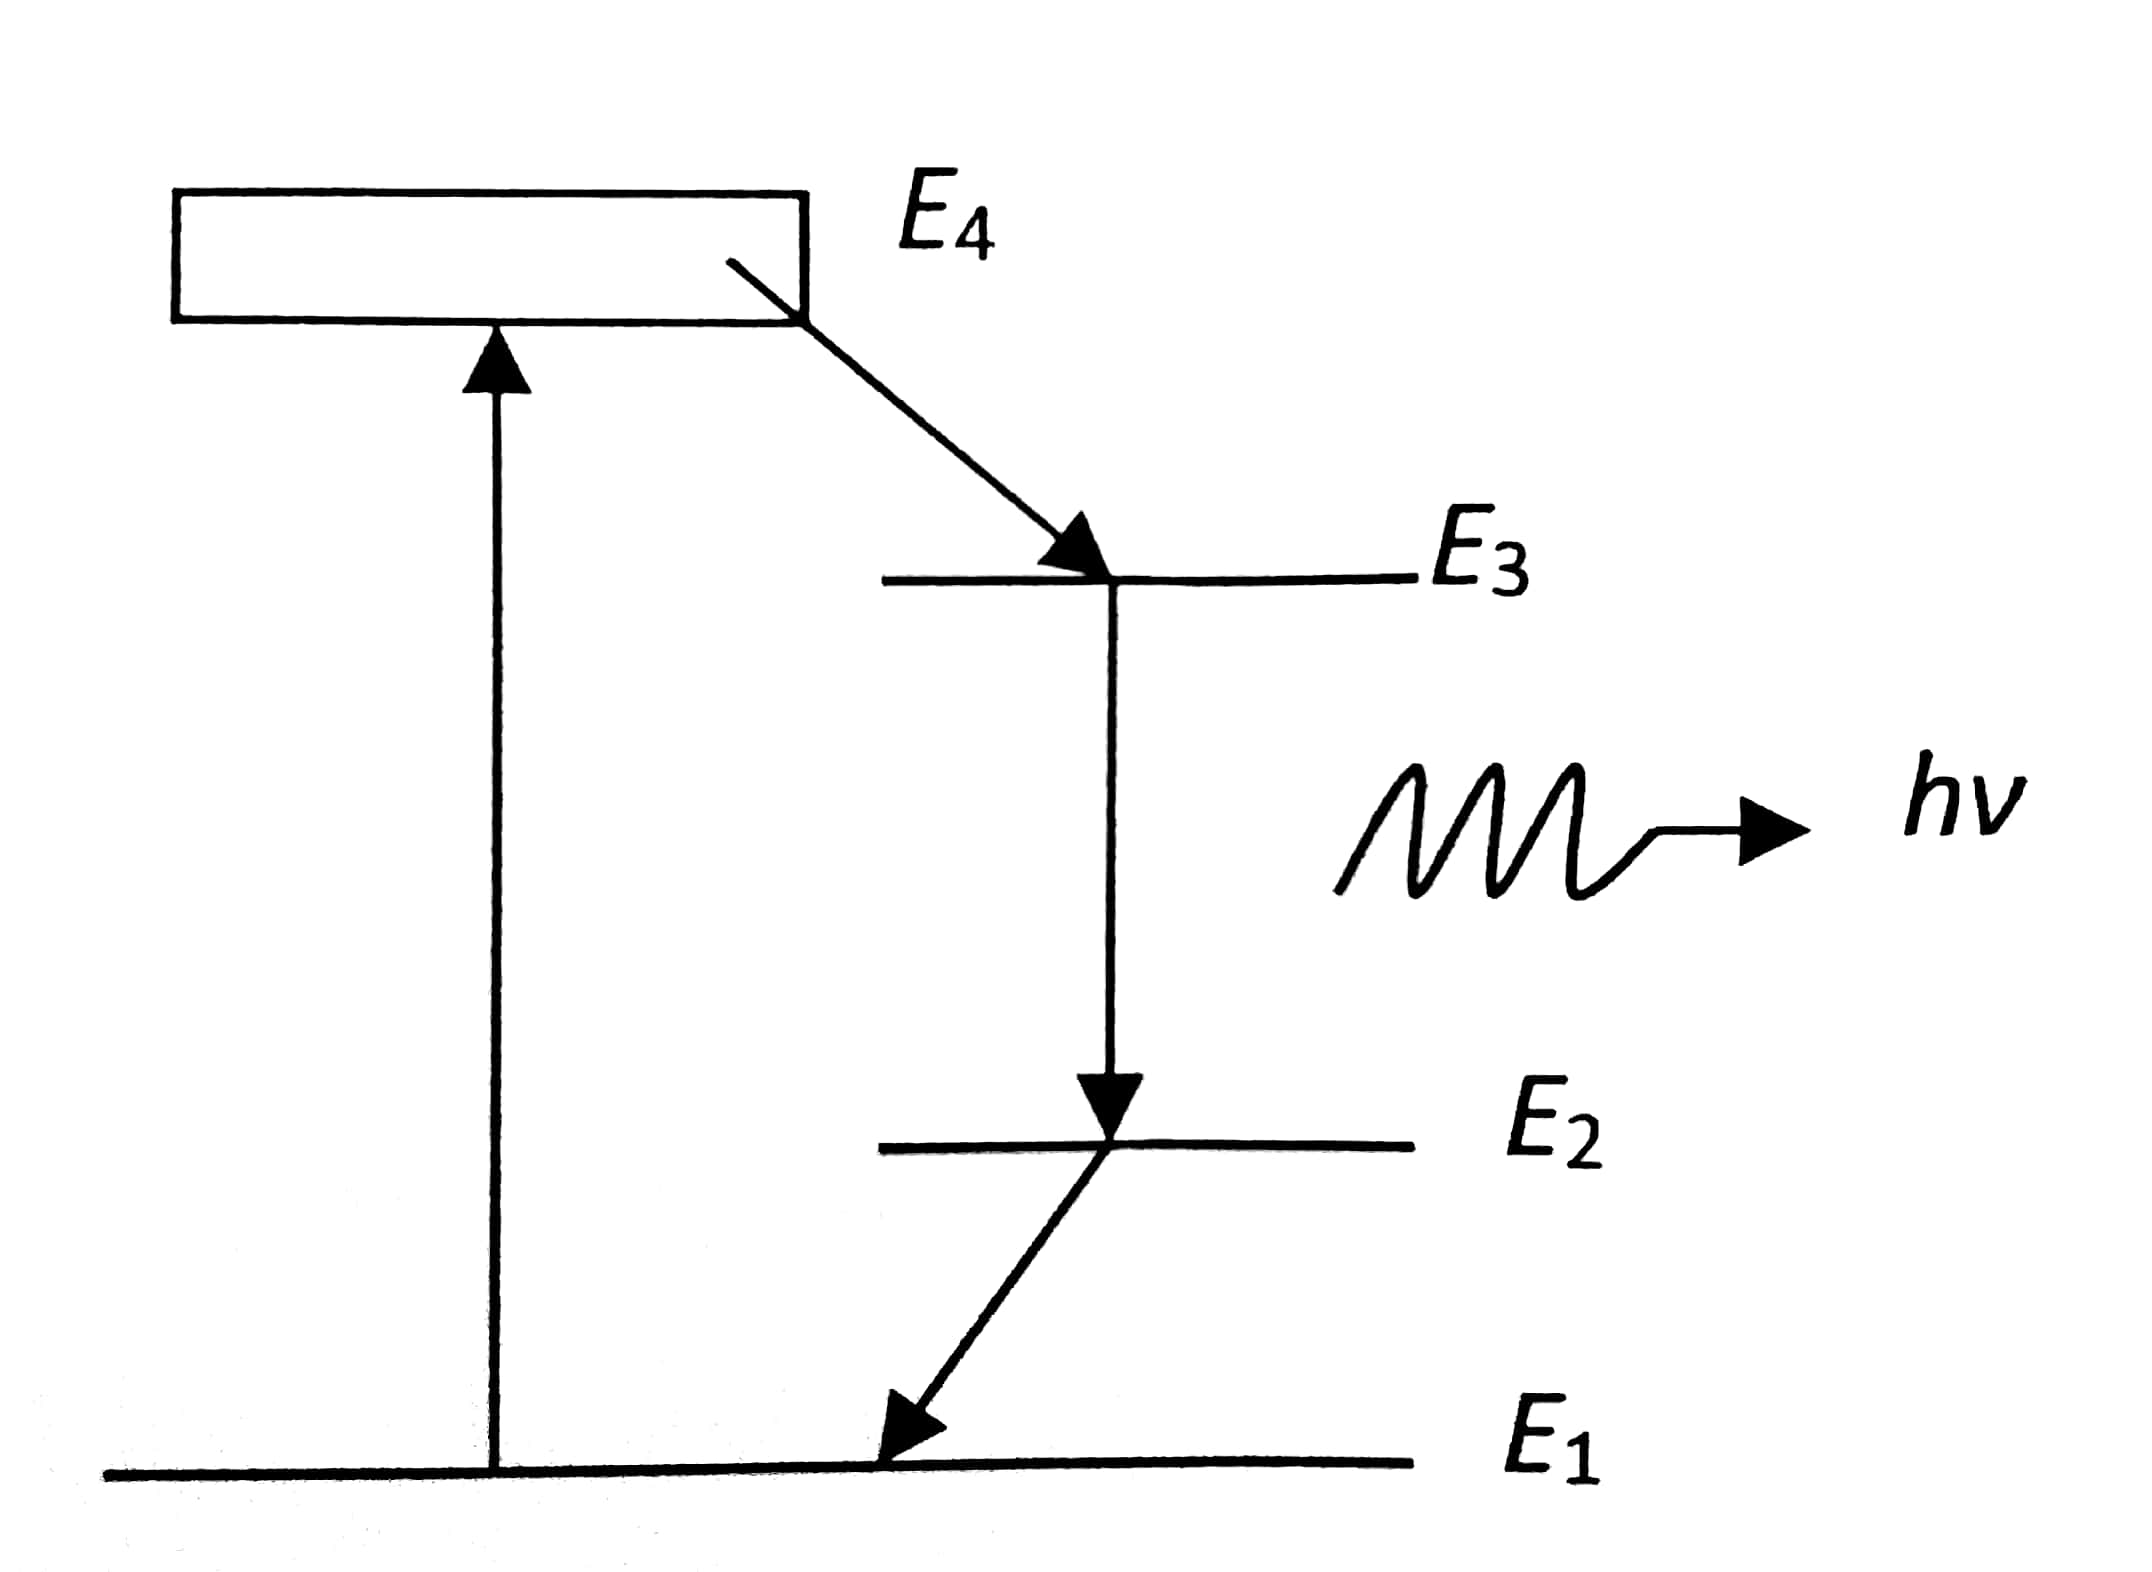
\includegraphics[height=3cm,width=4cm]{images/2.jpg}
    \label{fg2}
  \end{figure}
  \begin{itemize}
    \item 在光泵激励下,钕离子容易在\(\rm E_3\)和\(\rm E_2\)之间形成集聚数反转,实现受激辐射。
    \item 激光器形成自激震荡的条件是\(G^0 \times l \geq \alpha L \)
    \item 静态激光器输出的光脉冲为一群尖峰脉冲序列,称为激光弛豫震荡
  \end{itemize}
  
\end{frame}
\begin{frame}{实验原理}{调Q工作原理}
  \begin{itemize}
    \item 静态激光器因为弛豫震荡,输出功率受到限制。
    \item 采用调Q技术可以使激光能量集中到单脉冲,峰值功率可达兆瓦以上。
    \item 调Q晶体的吸收系数与入射光强之间的关系为:
    \begin{figure}
      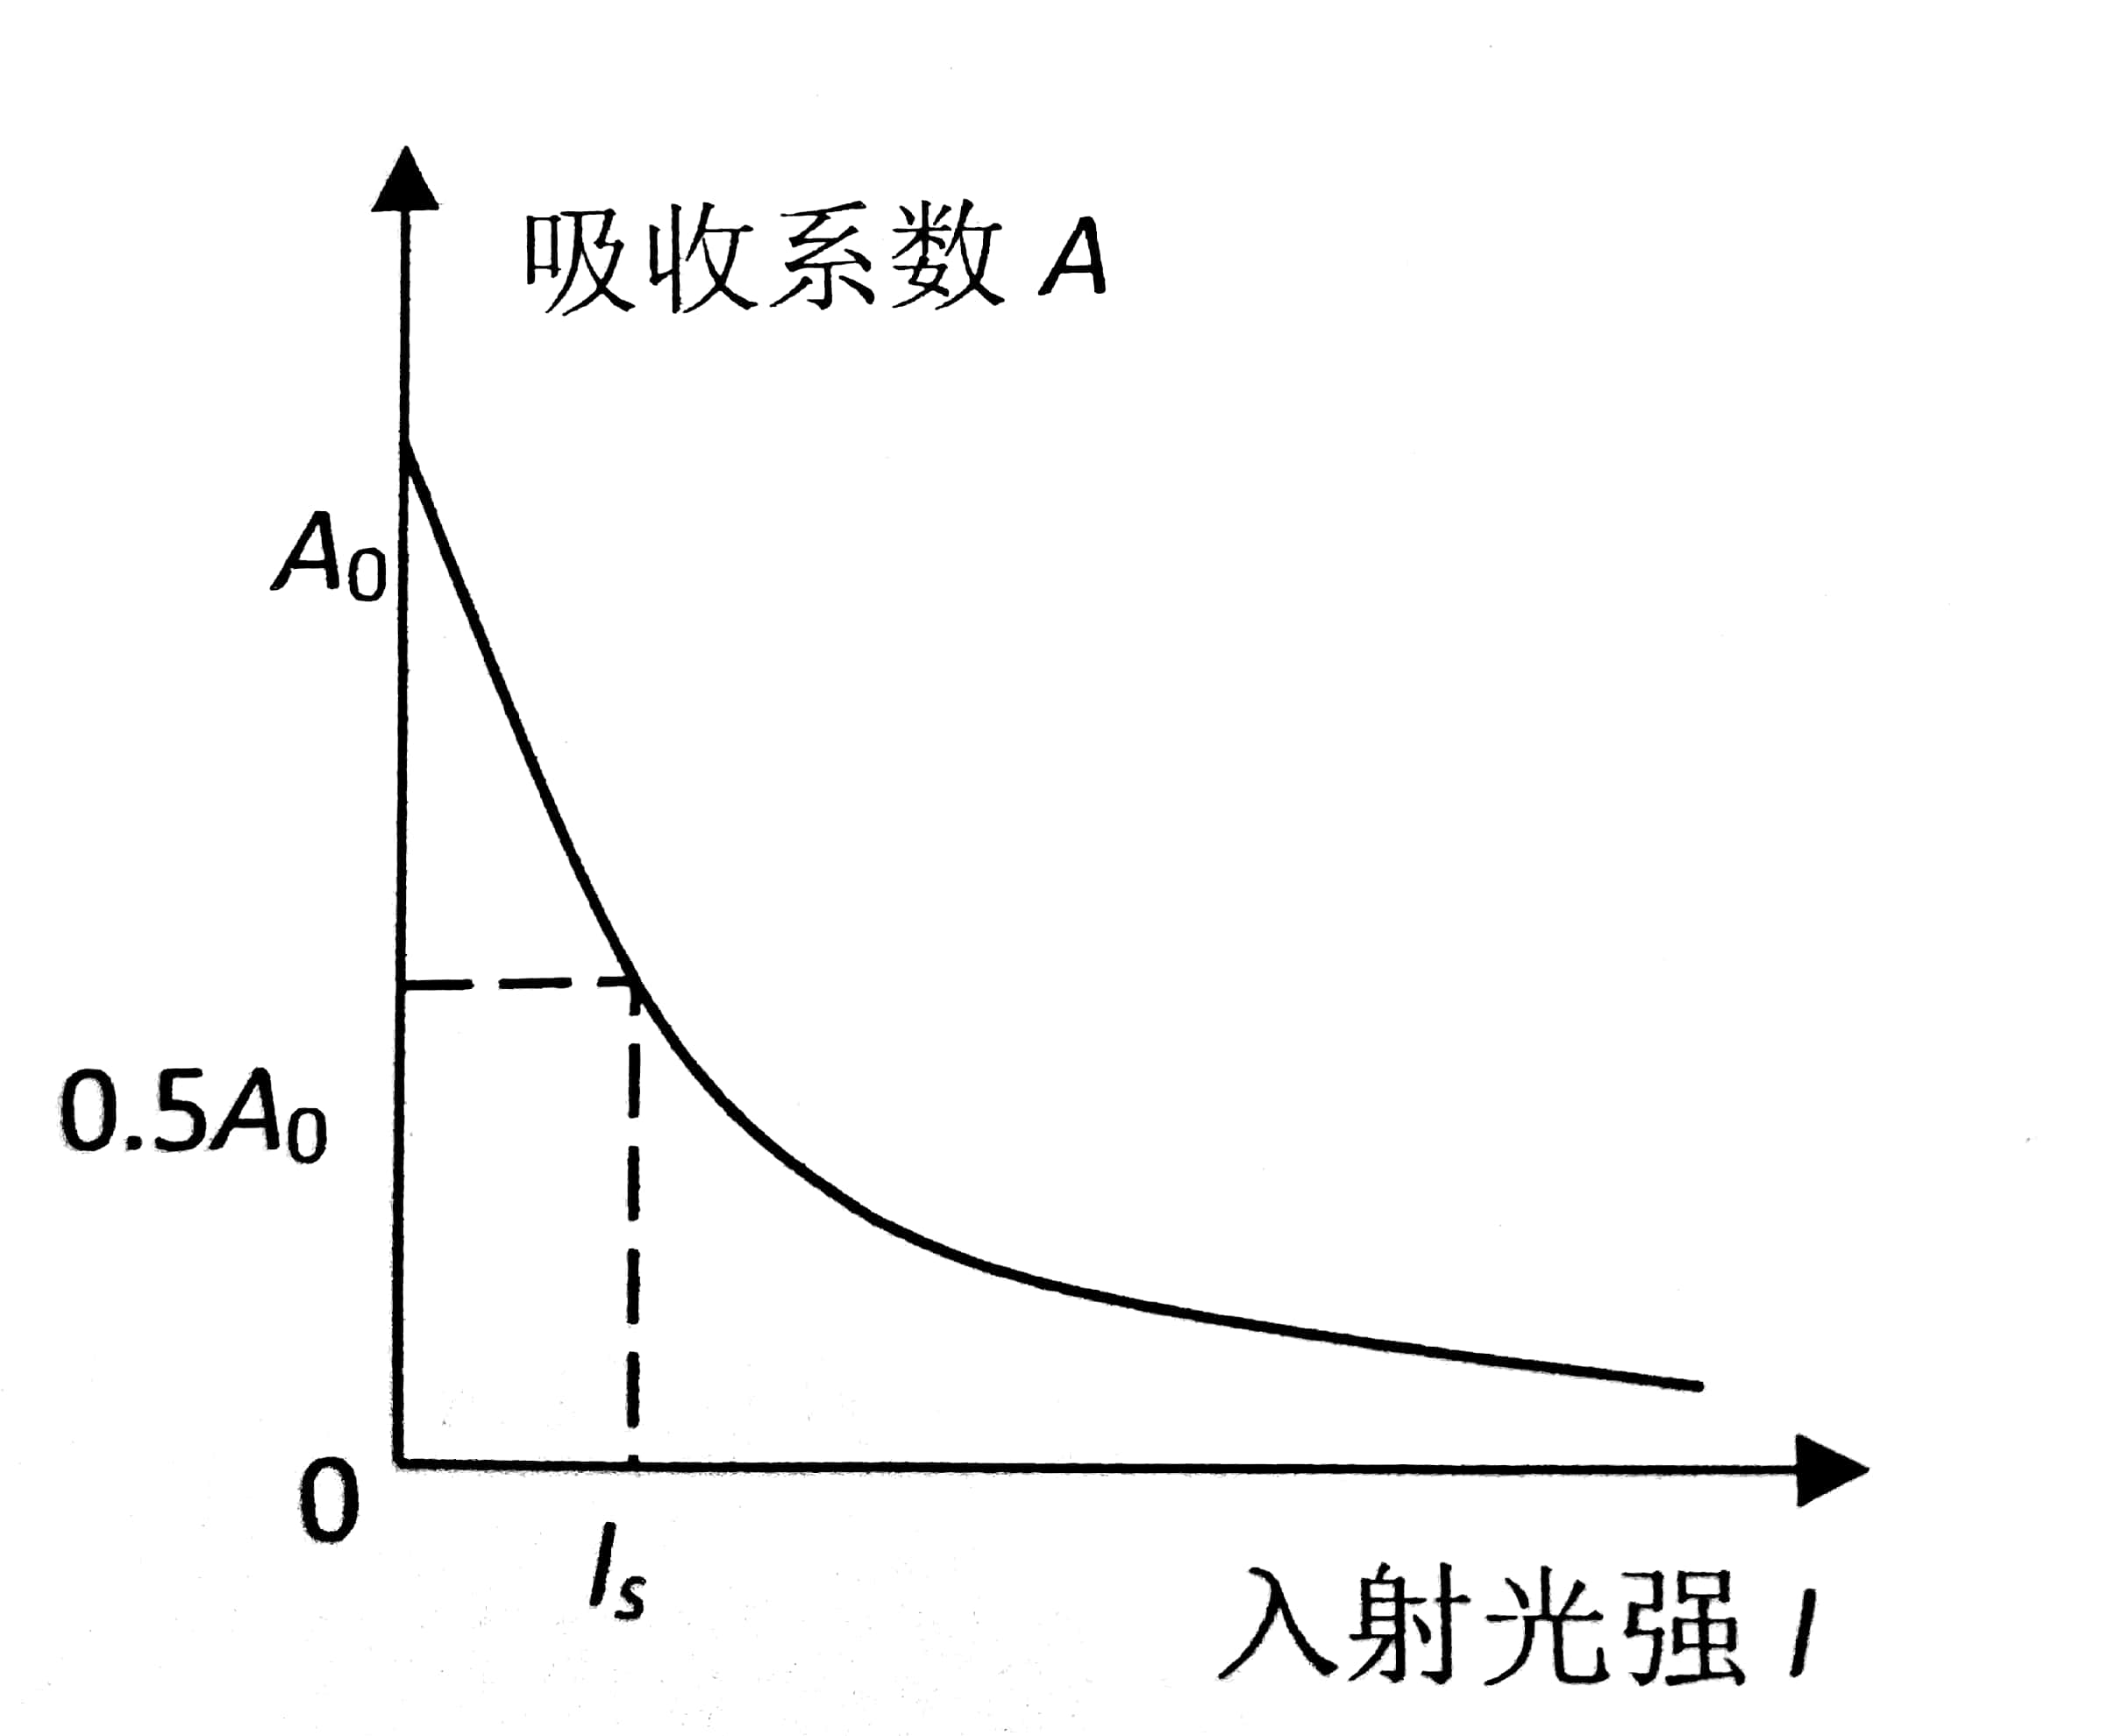
\includegraphics[height=3cm,width=4cm]{images/4.jpg}
      \label{fg2}
    \end{figure}
  \end{itemize}
  


  \begin{itemize}
    \item 光强较弱时,调Q吸收系数大,无法产生激光
    \item 光强增大到一定程度后,调Q吸收系数降低,受激辐射光强急剧增长
  \end{itemize}
  
\end{frame}

\begin{frame}{实验原理}{调Q工作原理}
  \begin{itemize}
    \item 燃料调Q激光器能量输出特性为:
    \begin{figure}
      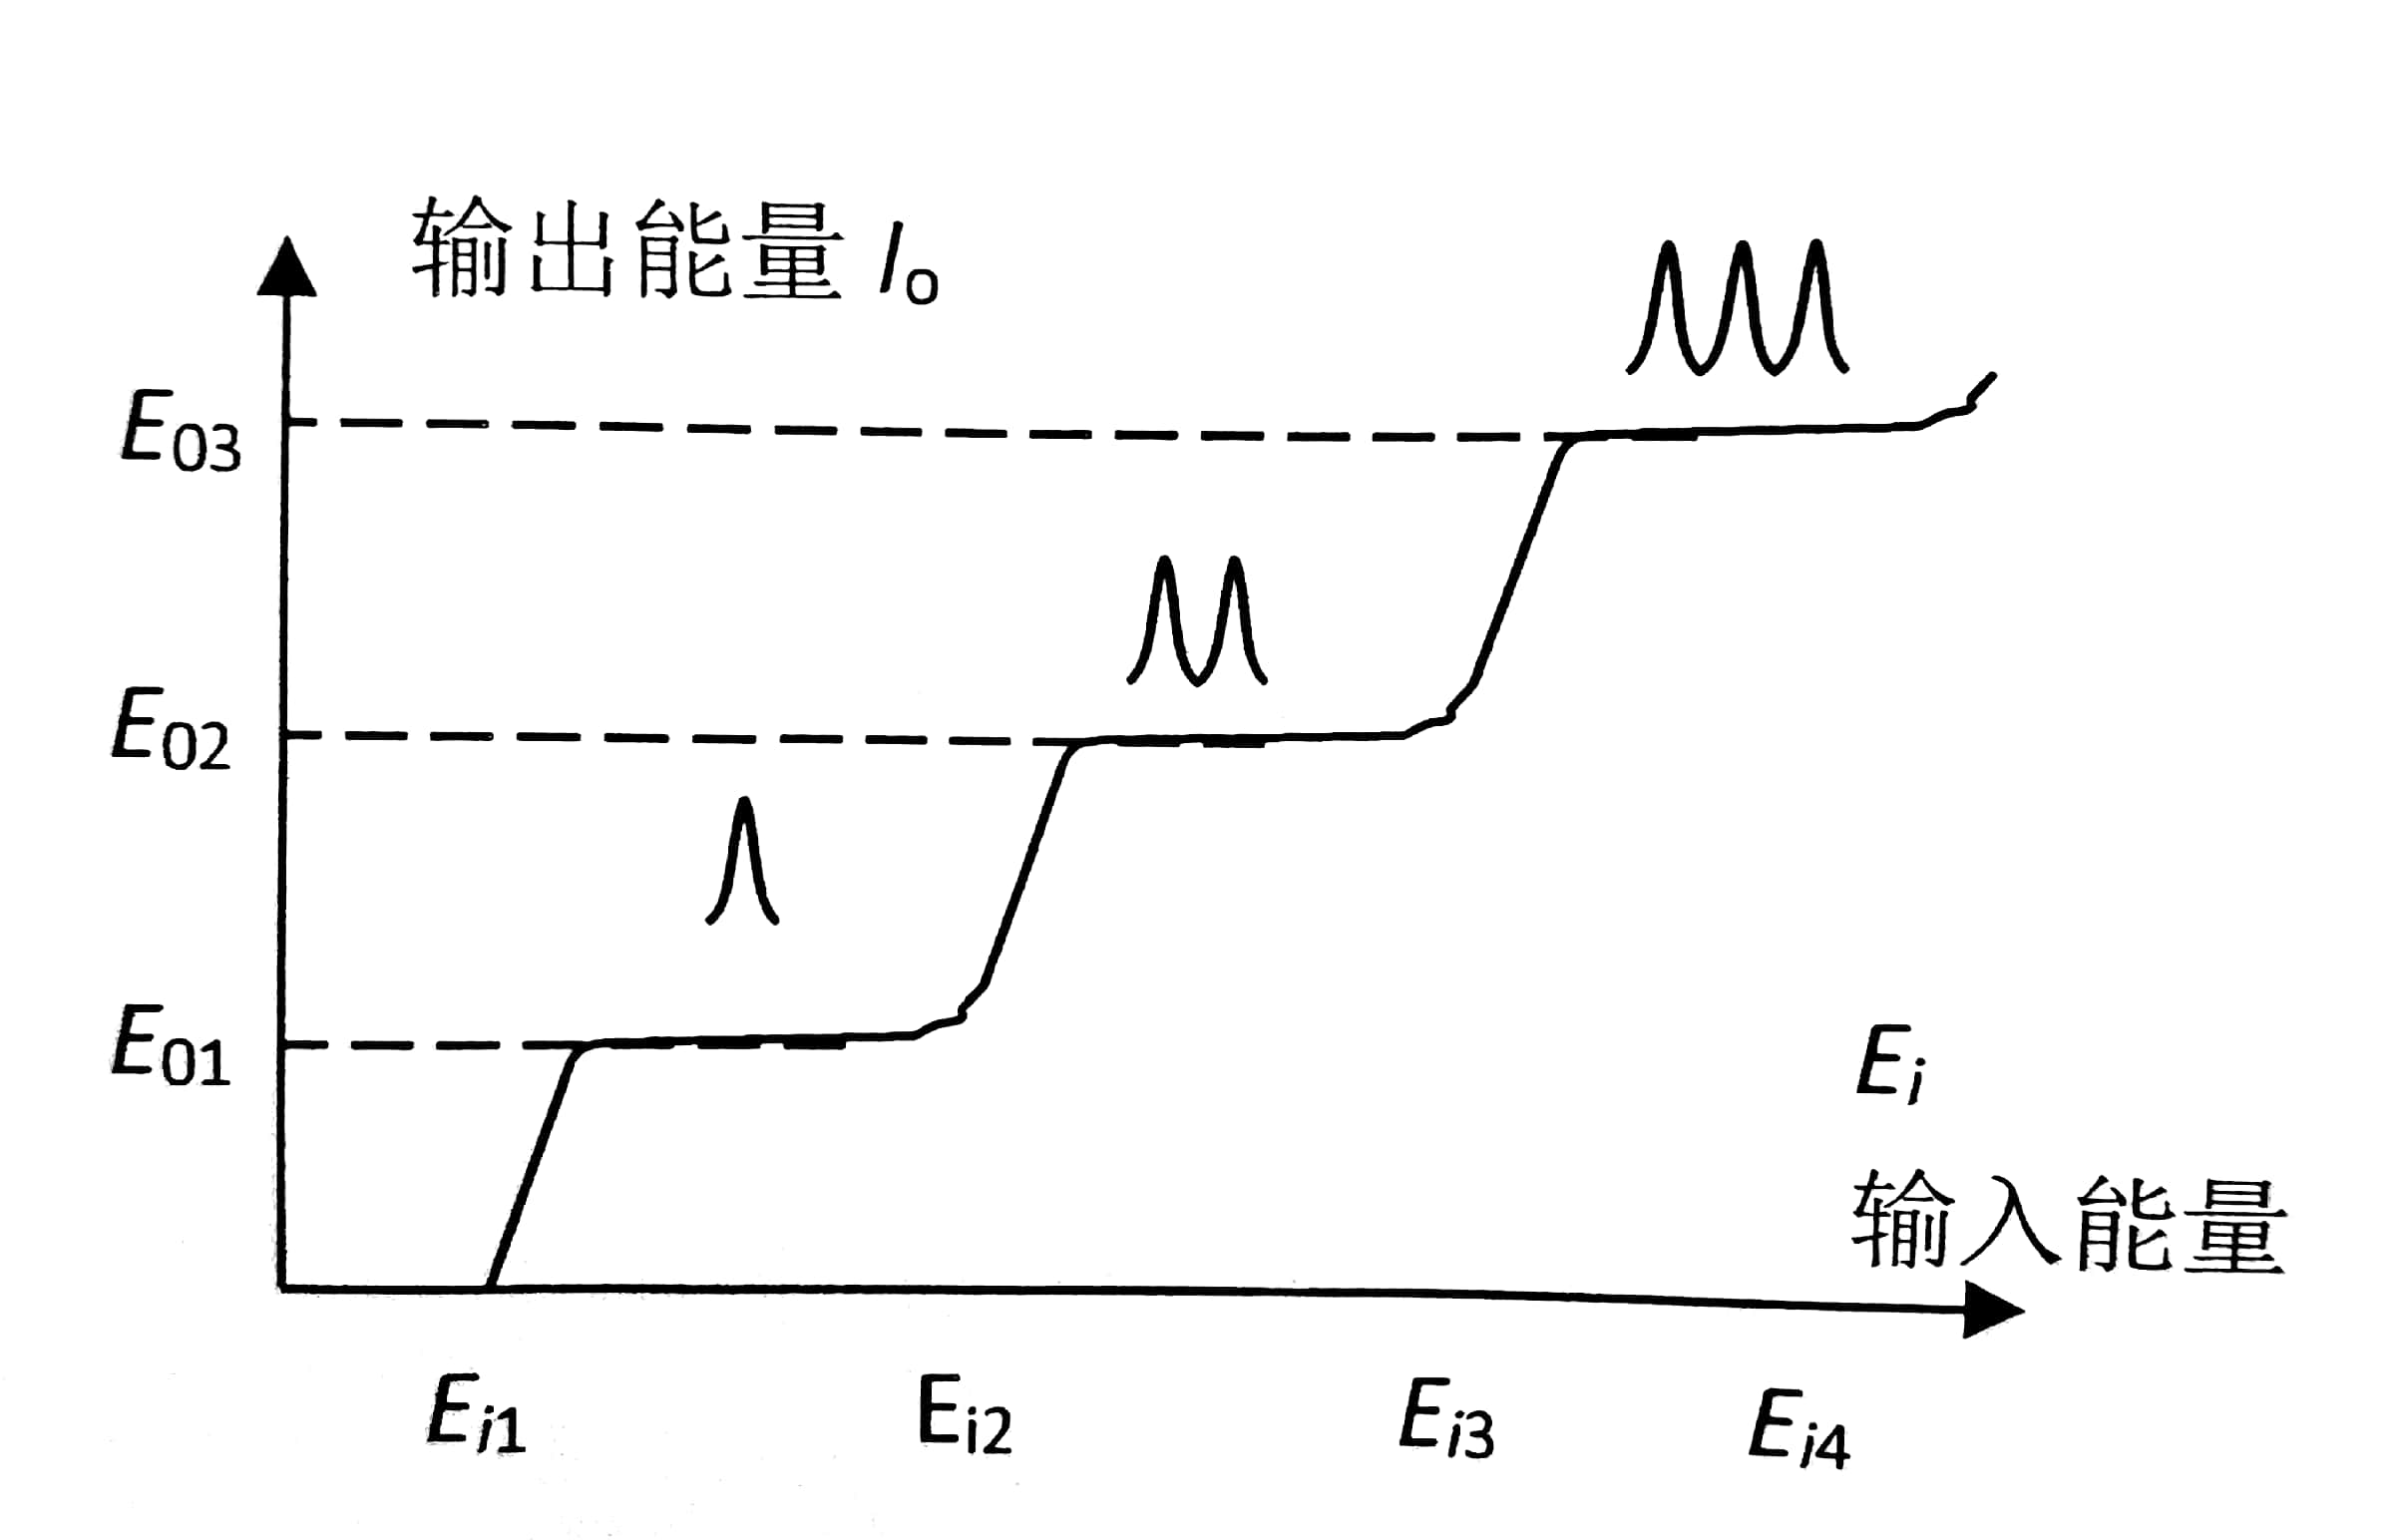
\includegraphics[height=3cm,width=4cm]{images/5.jpg}
      \label{fg2}
    \end{figure}
  \end{itemize}
  

\begin{block}{重要概念}
  \begin{itemize}
    \item 调Q晶体初始透过率
    \item 调Q效率/动静比
  \end{itemize}
\end{block}
  
\end{frame}


%---------------------------------------------------------
% 
%---------------------------------------------------------
\section{实验系统}
\section{方法步骤}
\section{实验结果}
\section{结果分析及结论}


\end{document}


% In this slide, some important text will be
% \alert{highlighted} beause it's important.
% Please, don't abuse it.

% \begin{block}{Remark}
% Sample text
% \end{block}

% \begin{alertblock}{Important theorem}
% Sample text in red box
% \end{alertblock}

% \begin{examples}
% Sample text in green box. "Examples" is fixed as block title.
% \end{examples}

%---------------------------------------------------------
%Two columns
% \begin{frame}
% \frametitle{Two-column slide}

% \begin{columns}

% \column{0.5\textwidth}
% This is a text in first column.
% $$E=mc^2$$
% \begin{itemize}
% \item First item
% \item Second item
% \end{itemize}

% \column{0.5\textwidth}
% This text will be in the second column
% and on a second tought this is a nice looking
% layout in some cases.
% \end{columns}
% \end{frame}